\usetikzlibrary{positioning, fit, backgrounds}
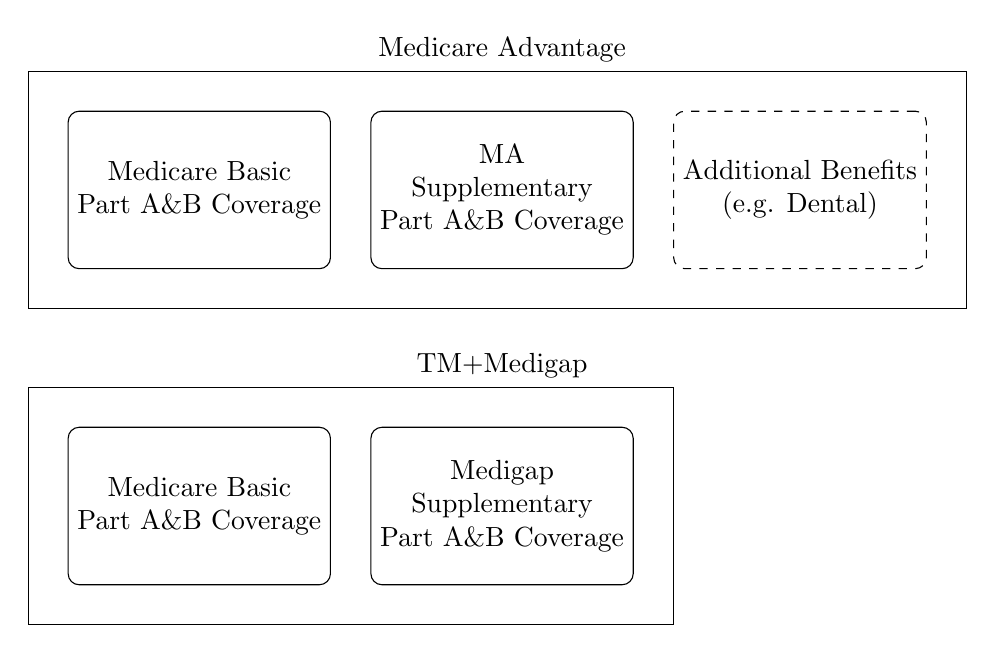
\begin{tikzpicture}[
    block/.style={
      draw,
      rectangle,
      rounded corners,
      minimum height=2cm, 
      minimum width=3cm, 
      align=center
    },
    node distance=0.5cm
]
% Nodes of MA coverage
\node[block] (ma) {Medicare Basic\\Part A\&B Coverage};
\node[block, right=of ma] (supp) {MA\\Supplementary\\Part A\&B Coverage};
% make the add node in dashed line
\node[block, right=of supp, dashed] (add) {Additional Benefits \\ (e.g. Dental)};

% group the nodes
\begin{scope}[on background layer]
    % add title MA Benefits over the nodes
  \node[above=0.5cm of supp] {Medicare Advantage};
  \node[fit=(ma) (supp) (add), draw, inner sep=0.5cm] (ma_group) {};
\end{scope}

% add space between the two groups
\node[below=1cm of ma_group] {};

% Nodes of Medigap coverage
\node[block, below=2cm of ma] (medigap) {Medicare Basic\\Part A\&B Coverage};
\node[block, right=of medigap] (medigap_supp) {Medigap\\Supplementary\\Part A\&B Coverage};


% group the nodes
\begin{scope}[on background layer]
    % add title Medigap Benefits over the nodes
  \node[above=0.5cm of medigap_supp] {TM+Medigap};
  \node[fit=(medigap) (medigap_supp), draw, inner sep=0.5cm] (medigap_group) {};
\end{scope}

\end{tikzpicture}